\documentclass[10pt,xcolor=x11names,compress, show notes]{beamer}% pour l'impression, tout n'apparait qu'une fois \documentclass[handout,12pt]{beamer}

%\usepackage[scaled]{helvet}
\usepackage[round]{natbib}
\usepackage[utf8x]{inputenc}
\usepackage[USenglish]{babel}
\usepackage{todonotes}
\usepackage{color}
\usepackage{pbox}
\usepackage{graphicx}


\usepackage{changepage}
\usepackage{pifont} %pour les symbole sympa \ding{nb}

\usepackage{subfig}

%%% Pour Tikz
\usepackage{tikz}
\usetikzlibrary{calc}
\usetikzlibrary{shapes}
%\usetikzlibrary{arrows,shapes,trees,positioning}  

%%%pour les plots matlab en tikz
\usepackage{pgfplots} 
\pgfplotsset{compat=newest}

%%% Pour les maths
\usepackage{bm}
\usepackage{amsmath,mathtools}
\usefonttheme[onlymath]{serif}
\usepackage{cancel} %pour barrer des math

%%% Pour la mise en forme
\usepackage[export]{adjustbox}
%\usepackage{subcaption}
\usepackage{wrapfig}
\usepackage{pdfpages}
\setbeamertemplate{navigation symbols}{} 
\usepackage{array}
%\usepackage{subfigure}
%\usepackage[]{geometry}
%\usepackage{palatino}
%\setbeamertemplate{caption}{\raggedright\insertcaption\par}
\usepackage{multicol}
\setlength{\columnsep}{0cm}
\usepackage[framemethod=TikZ]{mdframed}

\title{Introduction to Bayesian inference}
%%% Theme
\def \pied {~~~A. Dinsenmeyer~|~\insertshorttitle \hfill \insertframenumber/\inserttotalframenumber~~~} %content if footline
\usetheme{Alice}
\graphicspath{{./img/}}


\newcommand{\N}{\mathcal{N}}


\begin{document}

\begin{frame}
\maketitle
\end{frame}

%introduce machine learning with linear regression
\section{Introduction}
\begin{frame}{\insertsectionhead}
	\begin{center}
		$\bm{X}\cdot \bm{w} + \bm{b} = \bm{Y} $\\
		\includegraphics<1>[width=0.5\textwidth]{intro1.png}
		\includegraphics<2>[width=0.5\textwidth]{intro2.png}
	\end{center}
		In \textcolor{red}{\bfseries red} and \textcolor{cyan}{\bfseries blue} : unknown parameters that we have to learn\\
	
	\begin{itemize}	
		\item<1->\textbf{Classical regression }: \\
	find each parameter that best explain the data
	
		\item<2->\textbf{Going Bayesian }: \\
	Treat each parameter : random variable with other variable to be estimated. 
	\\e.g : mean + standard deviation
	         
	\end{itemize}
%	Ordinary least squares (no regularization)
%	Bayesian least squares
\vfill
{\scriptsize \textit{Image source :} \texttt{ericmjl.github.io/bayesian-deep-learning-demystified}}
\end{frame}

\begin{frame}{\insertsectionhead}
\vspace{-0.5cm}
\begin{minipage}{0.47\textwidth}
	\centering
	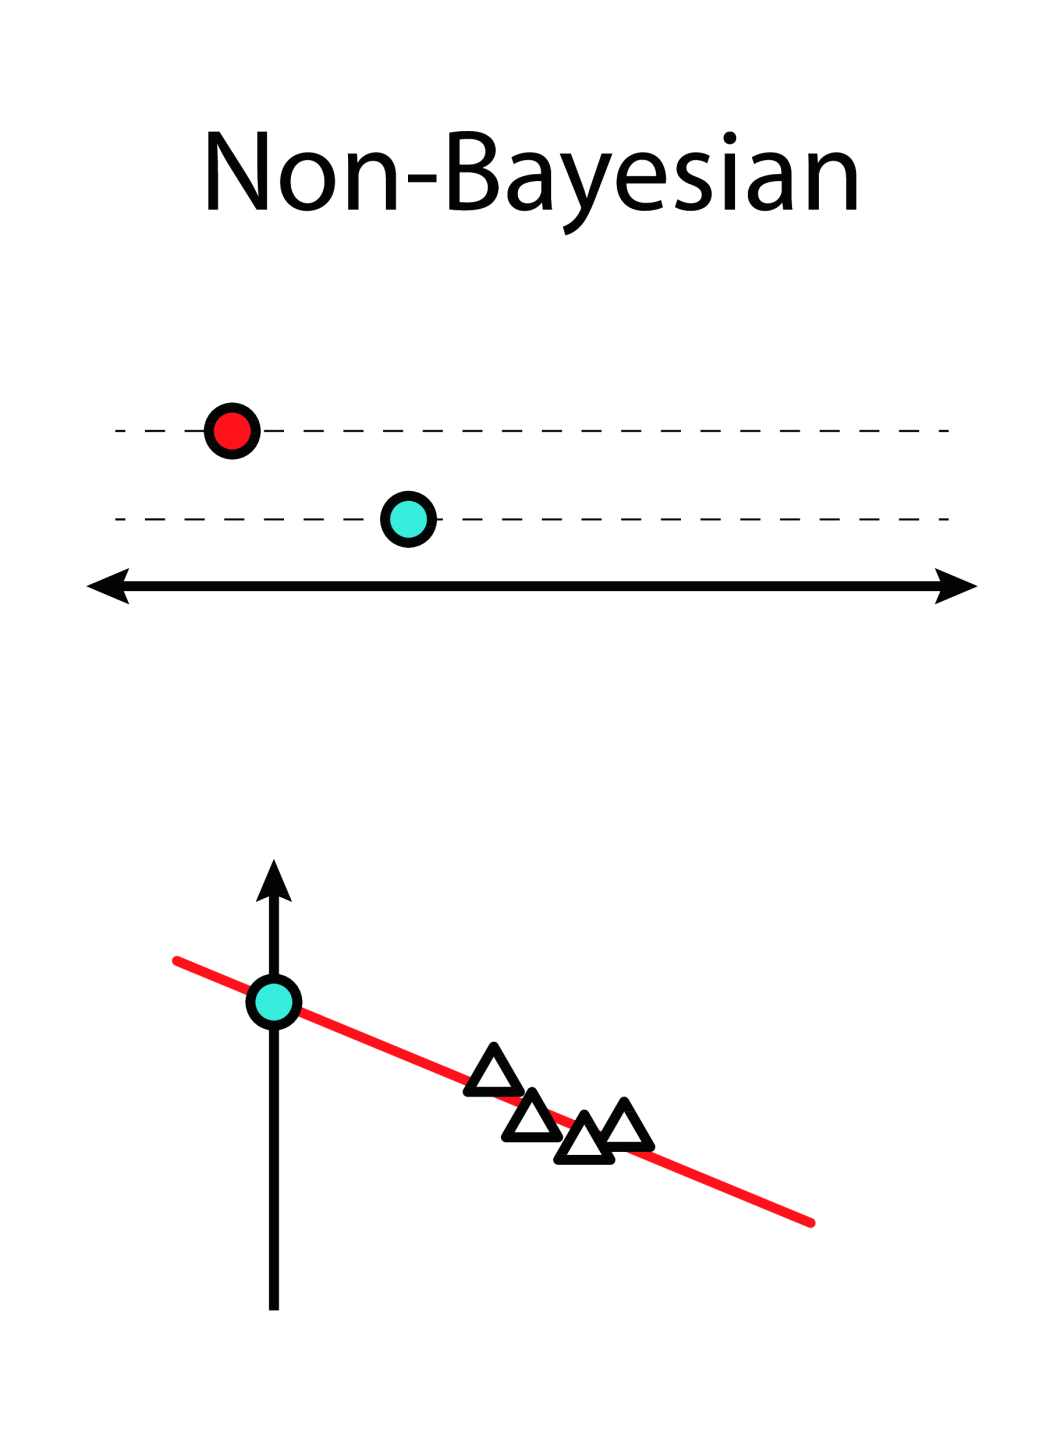
\includegraphics[height=0.7\textwidth]{linreg1.png}\\
\vfill
	Inferred parameters:\\ 1 \textcolor{red}{slope} + 1 \textcolor{cyan}{intercept}\\
	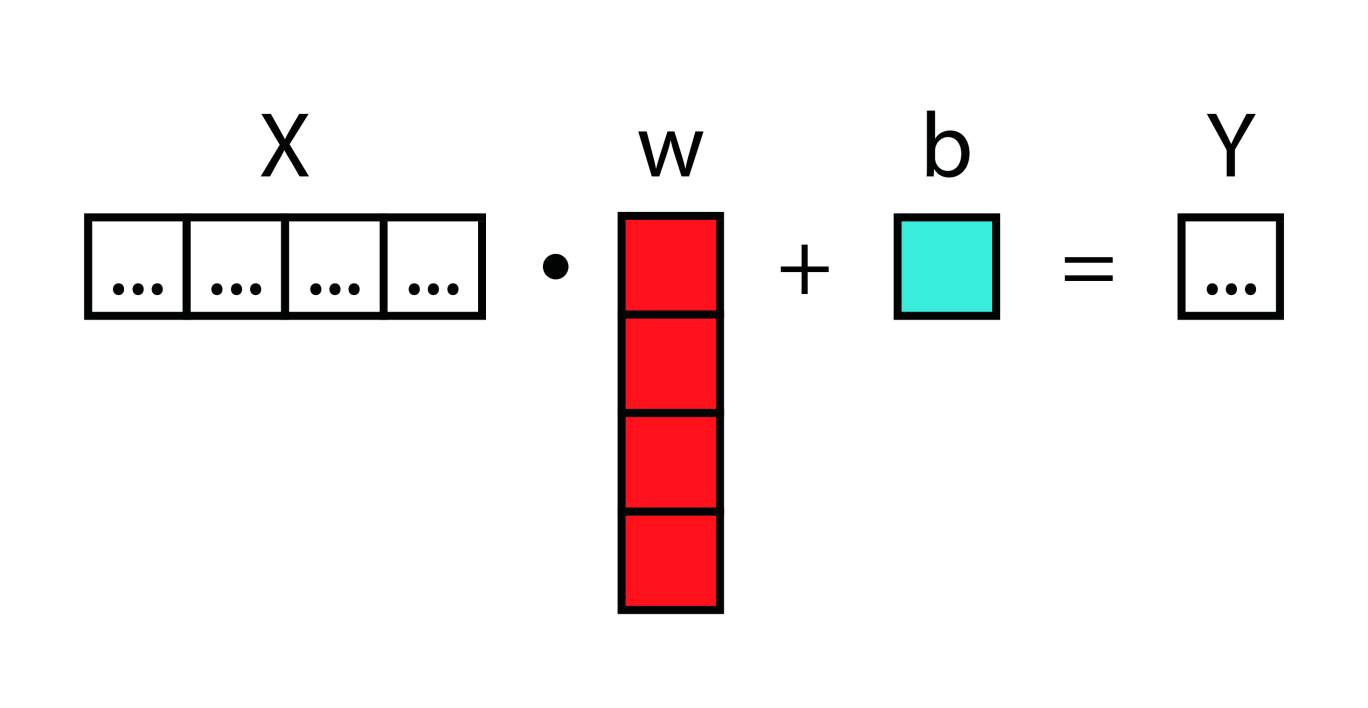
\includegraphics[width=0.7\textwidth]{intro1.png}\\
	
\end{minipage}
 \hfill 
 \onslide<2->\begin{minipage}{0.52\textwidth}
 	\centering
	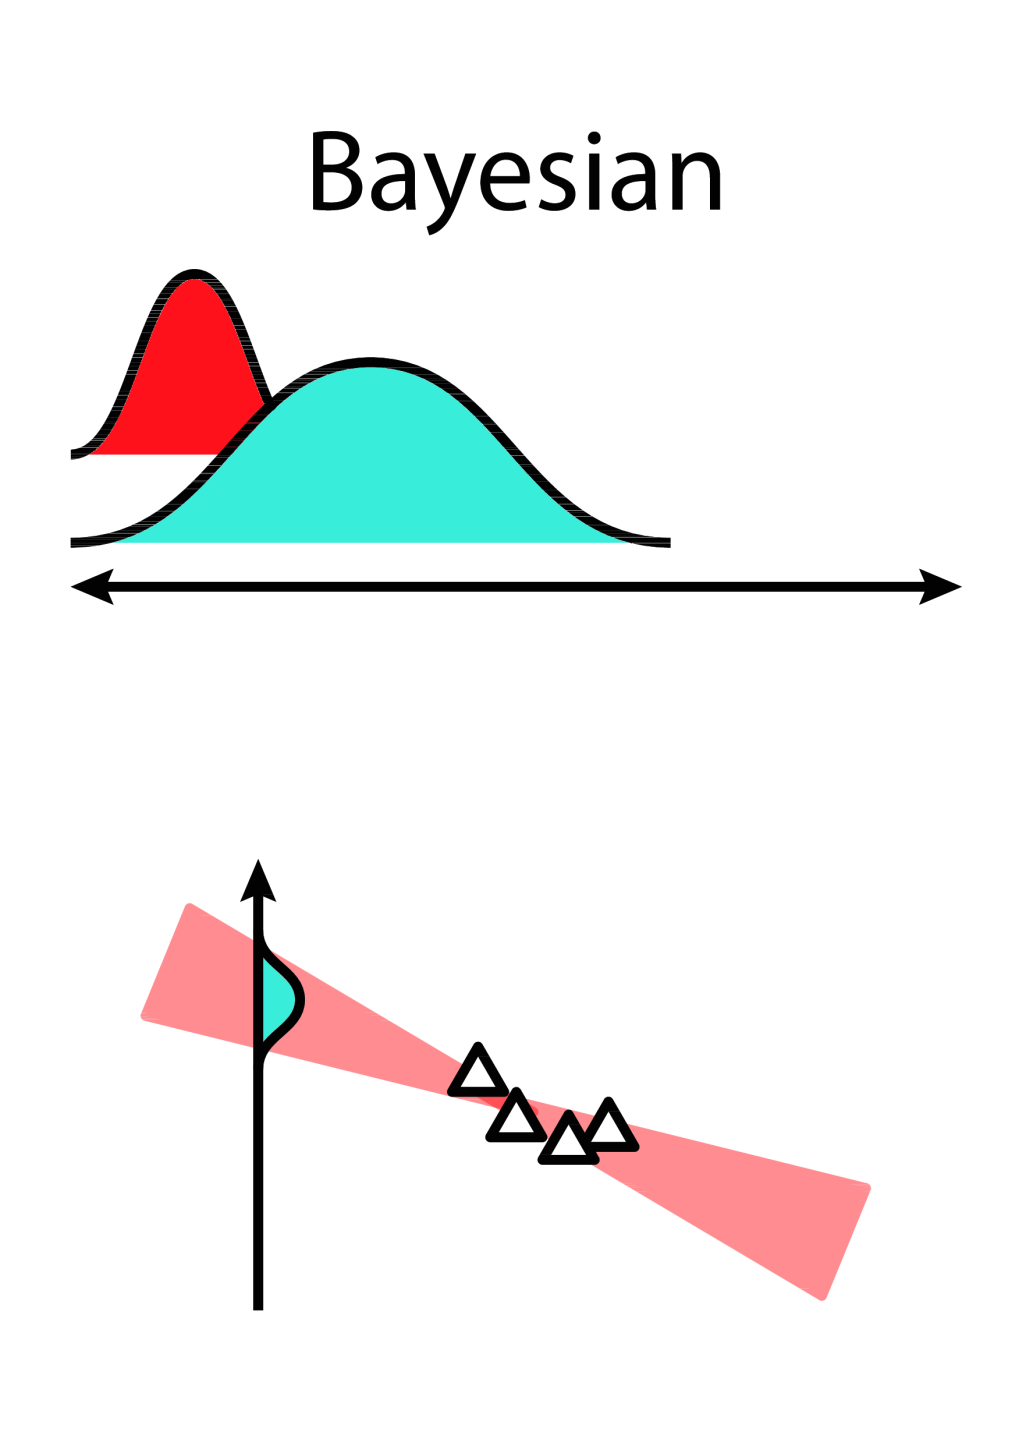
\includegraphics[height=0.7\textwidth]{linreg2.png}\\
	\vfill
	Inferred parameters:\\
	family of \textcolor{red}{slopes} + family of \textcolor{cyan}{intercepts}\\
	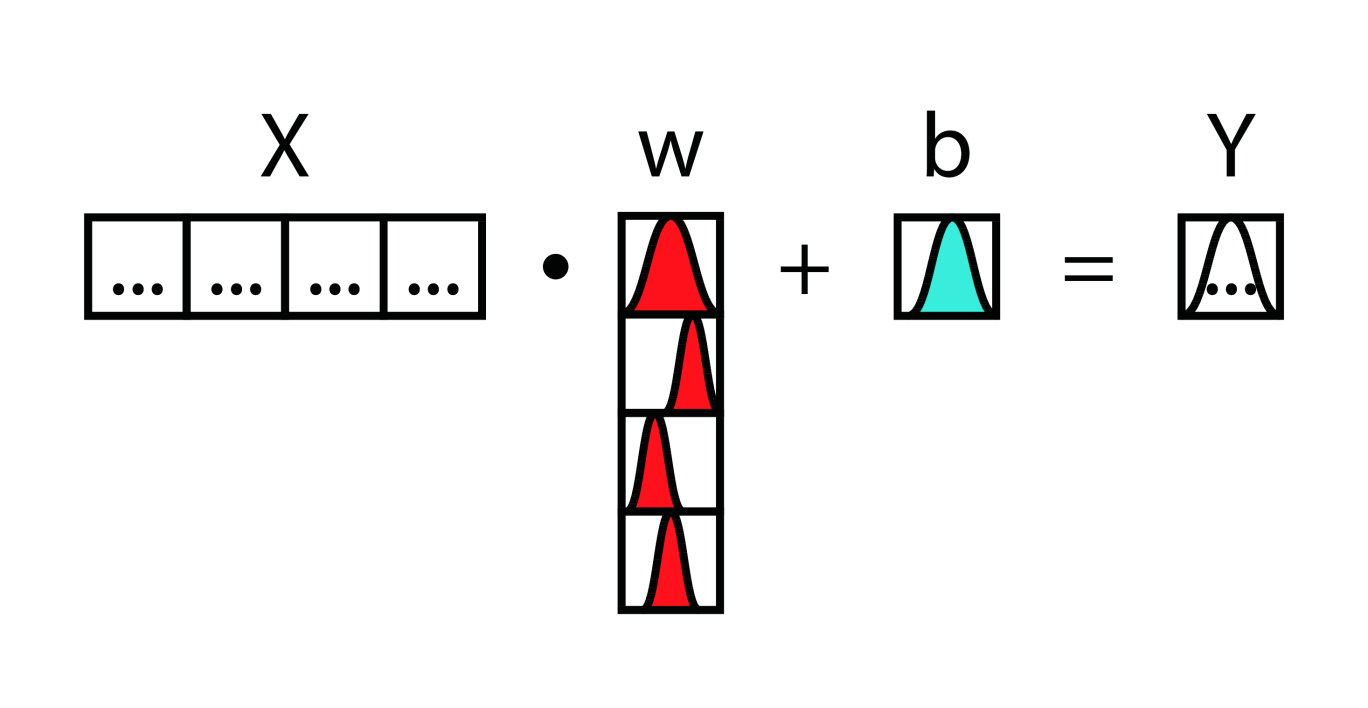
\includegraphics[width=0.7\textwidth]{intro2.png}\\
	{ $\hookrightarrow$ propagates the uncertainties}
	\vfill
\end{minipage}\\
\vfill
\begin{center}
	\footnotesize \textit{Image source :} \texttt{ericmjl.github.io/bayesian-deep-learning-demystified}
\end{center}
\end{frame}


\newcommand{\h}{\text{hypothesis}}
\renewcommand{\d}{\text{data}}
\newcommand{\p}{\text{parameters}}

\section{The Bayes rule}
\begin{frame}{\insertsectionhead}
\centering
\vspace{-1cm}
\textcolor{colorAlice}{\textbf{How to do inference about hypothesis from data ?}}\\


\alt<1>{$$ P(\h \mid \d) = \frac{P(\d \mid \h) P(\h)}{P(\d)}$$}{$$ P(\p \mid \d) = \frac{P(\d \mid \p) P(\p)}{P(\d)}$$}

\begin{overlayarea}{1.1\textwidth}{0.5\textheight}
\only<1-2>{\textbf{Required tools} : \\~\\
\begin{columns}
\begin{column}{0.4\textwidth}
	\centering
  Sum rule: $$ P(x) = \sum_y P(x,y)$$
\end{column}
\begin{column}{0.4\textwidth} 
	\centering
    Product rule: $$P(x,y)=P(x \mid y)P(y)$$
\end{column}
\end{columns}
}
\only<3-6>{
\pause \pause
\begin{itemize}
        \item $P(\d \mid \p)$: \textbf{likelihood }of a set of parameters in a given model \pause
        \item $P(\p)$ : \textbf{ prior }probability of the parameters\pause
        \item $P(\p \mid \d)$ : \textbf{posterior }probability of the parameter given the data\pause
        \item $P(\d)$ : \textbf{evidence} of the data\pause
\end{itemize}
}

\onslide<7->{
\textbf{Learning} : Use the data and the modelling assumption to transform what I knew before the data (prior) $\rightarrow$ gives the posterior\\~\\
\begin{minipage}[t]{0.50\textwidth}
\centering
        $\bullet$ classification / clustering\\
       {\small  (yes/no category)  (group similar things)}\\
        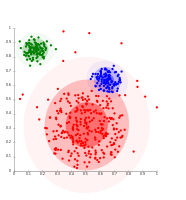
\includegraphics[width=0.5\linewidth]{clustering.png}\\
        {\scriptsize source : wikipedia}
\end{minipage}
\hfill
\begin{minipage}[t]{0.49\textwidth}
\centering
        $\bullet$ regression (predict values)\\
        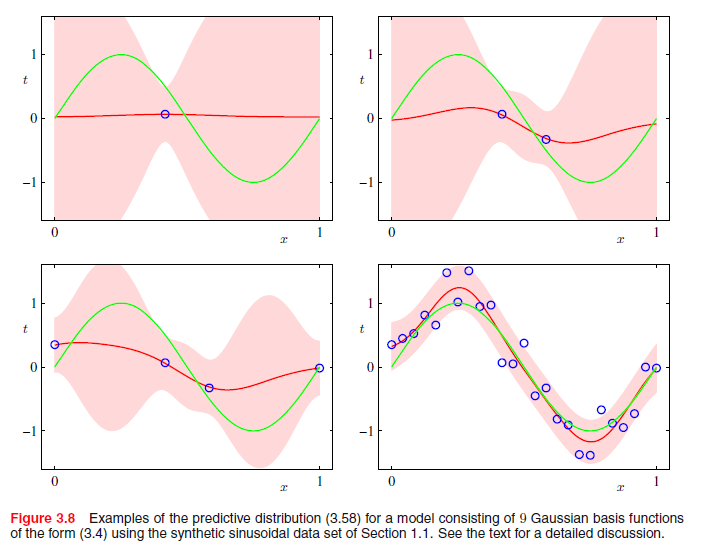
\includegraphics[width =0.5\linewidth]{regression.png}\\
        {\scriptsize source : Bishop, Pattern Recognition And Machine Learning}
\end{minipage}
}
\vfill
\end{overlayarea}

\end{frame}
\begin{frame}{\insertsectionhead}

\textbf{Bayes' rule is a way to infer parameter given underlying data}\\

$\hookrightarrow$ Bayesian machine learning is nothing more than learning a probability distribution for each parameter
\begin{center}
%\includegraphics<1>[width=0.8\textwidth]{intro1.png}
\includegraphics<1->[width=0.8\textwidth]{intro2.png}\\
{\scriptsize \textit{Image source :} \texttt{ericmjl.github.io/bayesian-deep-learning-demystified}}
\end{center}

\end{frame}

\section{Bayesian Machine Learning}
\begin{frame}{\insertsectionhead (in one slide)}
\begin{itemize}
        \item Have a model $\mathcal{M}(\theta)$ \pause
        \item Specify prior believes we have about the parameters $\theta$ \pause
        \item Observe the data \pause
        \item Compute the posterior $P(\theta \mid \text{data})$ \pause
        \item Repeat for multiple models/parameter \pause
        \item See which model(s)/parameter(s) fit for your data. \pause
\end{itemize}
\end{frame}

\section{Linear regression}
\begin{frame}{\insertsectionhead}	
\textbf{Example with $\ell_2$ cost (linear least square problem) }:
\vfill
The objective function is : $$ f = \frac{1}{2}\| y-\hat{y}  \|^2_2$$
with $\ell_2$ regularization : $$ f = \frac{1}{2}\|y- \hat{y}  \|^2_2 + \frac{\lambda}{2}\|w\|^2_2$$ 
with the model $\hat{y}= Xw$
\end{frame}
\begin{frame}{\insertsectionhead}
\textbf{Frequentist statistics point of view} :
$$y = \hat{y} + \epsilon$$
Let's model $\hat{y}$ as a Gaussian random variable : $\hat{y} \sim \N(\mu,\sigma^2)$ with $\mu = \hat{y} = Xw$ (the prediction of the model). 
\begin{align}
P(y \mid X,w,\sigma^2)& = \N(Xw, \sigma^2) \hfill \rightarrow\text{likelihood}\\
&= \frac{1}{\sqrt{2\pi \sigma^2}}\exp\left(-\frac{(y-Xw)^2}{2 \sigma^2} \right)
\end{align}
~\\
\pause
 \textit{Maximum Likelihood Estimate} : $\boxed{w_{\text{\textsc{mle}}} = \arg\max \N(Xw, \sigma^2)}$\\~\\
 \pause
 or, minimizing the neg-log likelihood : 
 $$\boxed{w_{\text{\textsc{mle}}} = \arg\min (y - Xw)^2}$$
 
 $\hookrightarrow$ MLE on Gaussian Likelihood is equivalent to the least squares
\end{frame}

\begin{frame}{\insertsectionhead}
	\textbf{Bayesian point of view}\\
	We introduce the prior and then maximize the posterior:
	$$\underbrace{P(w \mid y,X)}_{\text{posterior}}\propto \underbrace{P(y,X,w)}_{\text{likelihood}}\underbrace{P(w \mid \mu_w,\sigma^2_{w})}_{\text{prior}}$$
	\pause
	Gaussian prior for $w$ : $P(w \mid \mu_w,\sigma^2_w) = \N(0,\sigma_0)$,
	$$P(w \mid y,X) \propto \exp\left(-\frac{(y-Xw)^2}{\sigma^2}	\right) \exp \left(-\frac{(w-\mu_w)^2}{\sigma^2_w} \right)$$
	\pause ~\\
	Then, minimize the neg-log posterior writes:
	$$w_{\text{\textsc{MAP}}} = \arg\min \| \hat{y}-Xw\|^2_2 + \lambda \|w\|^2_2$$
	$\hookrightarrow$ Gaussian prior leads to $\ell_2$ regularization.\\~\\

\begin{center}
\footnotesize
	\textit{$\bullet$ Note 1: if the prior on $w$ is uniform (non informative prior), \\
	Maximum a Posteriori =  Maximum Likelihood estimate}\\~\\
	
	\textit{$\bullet$ Note 2:  good informative prior $\rightarrow$  efficient regularization}
	\end{center}
\end{frame}


\begin{frame}{How the prior drives the posterior}
	\centering
	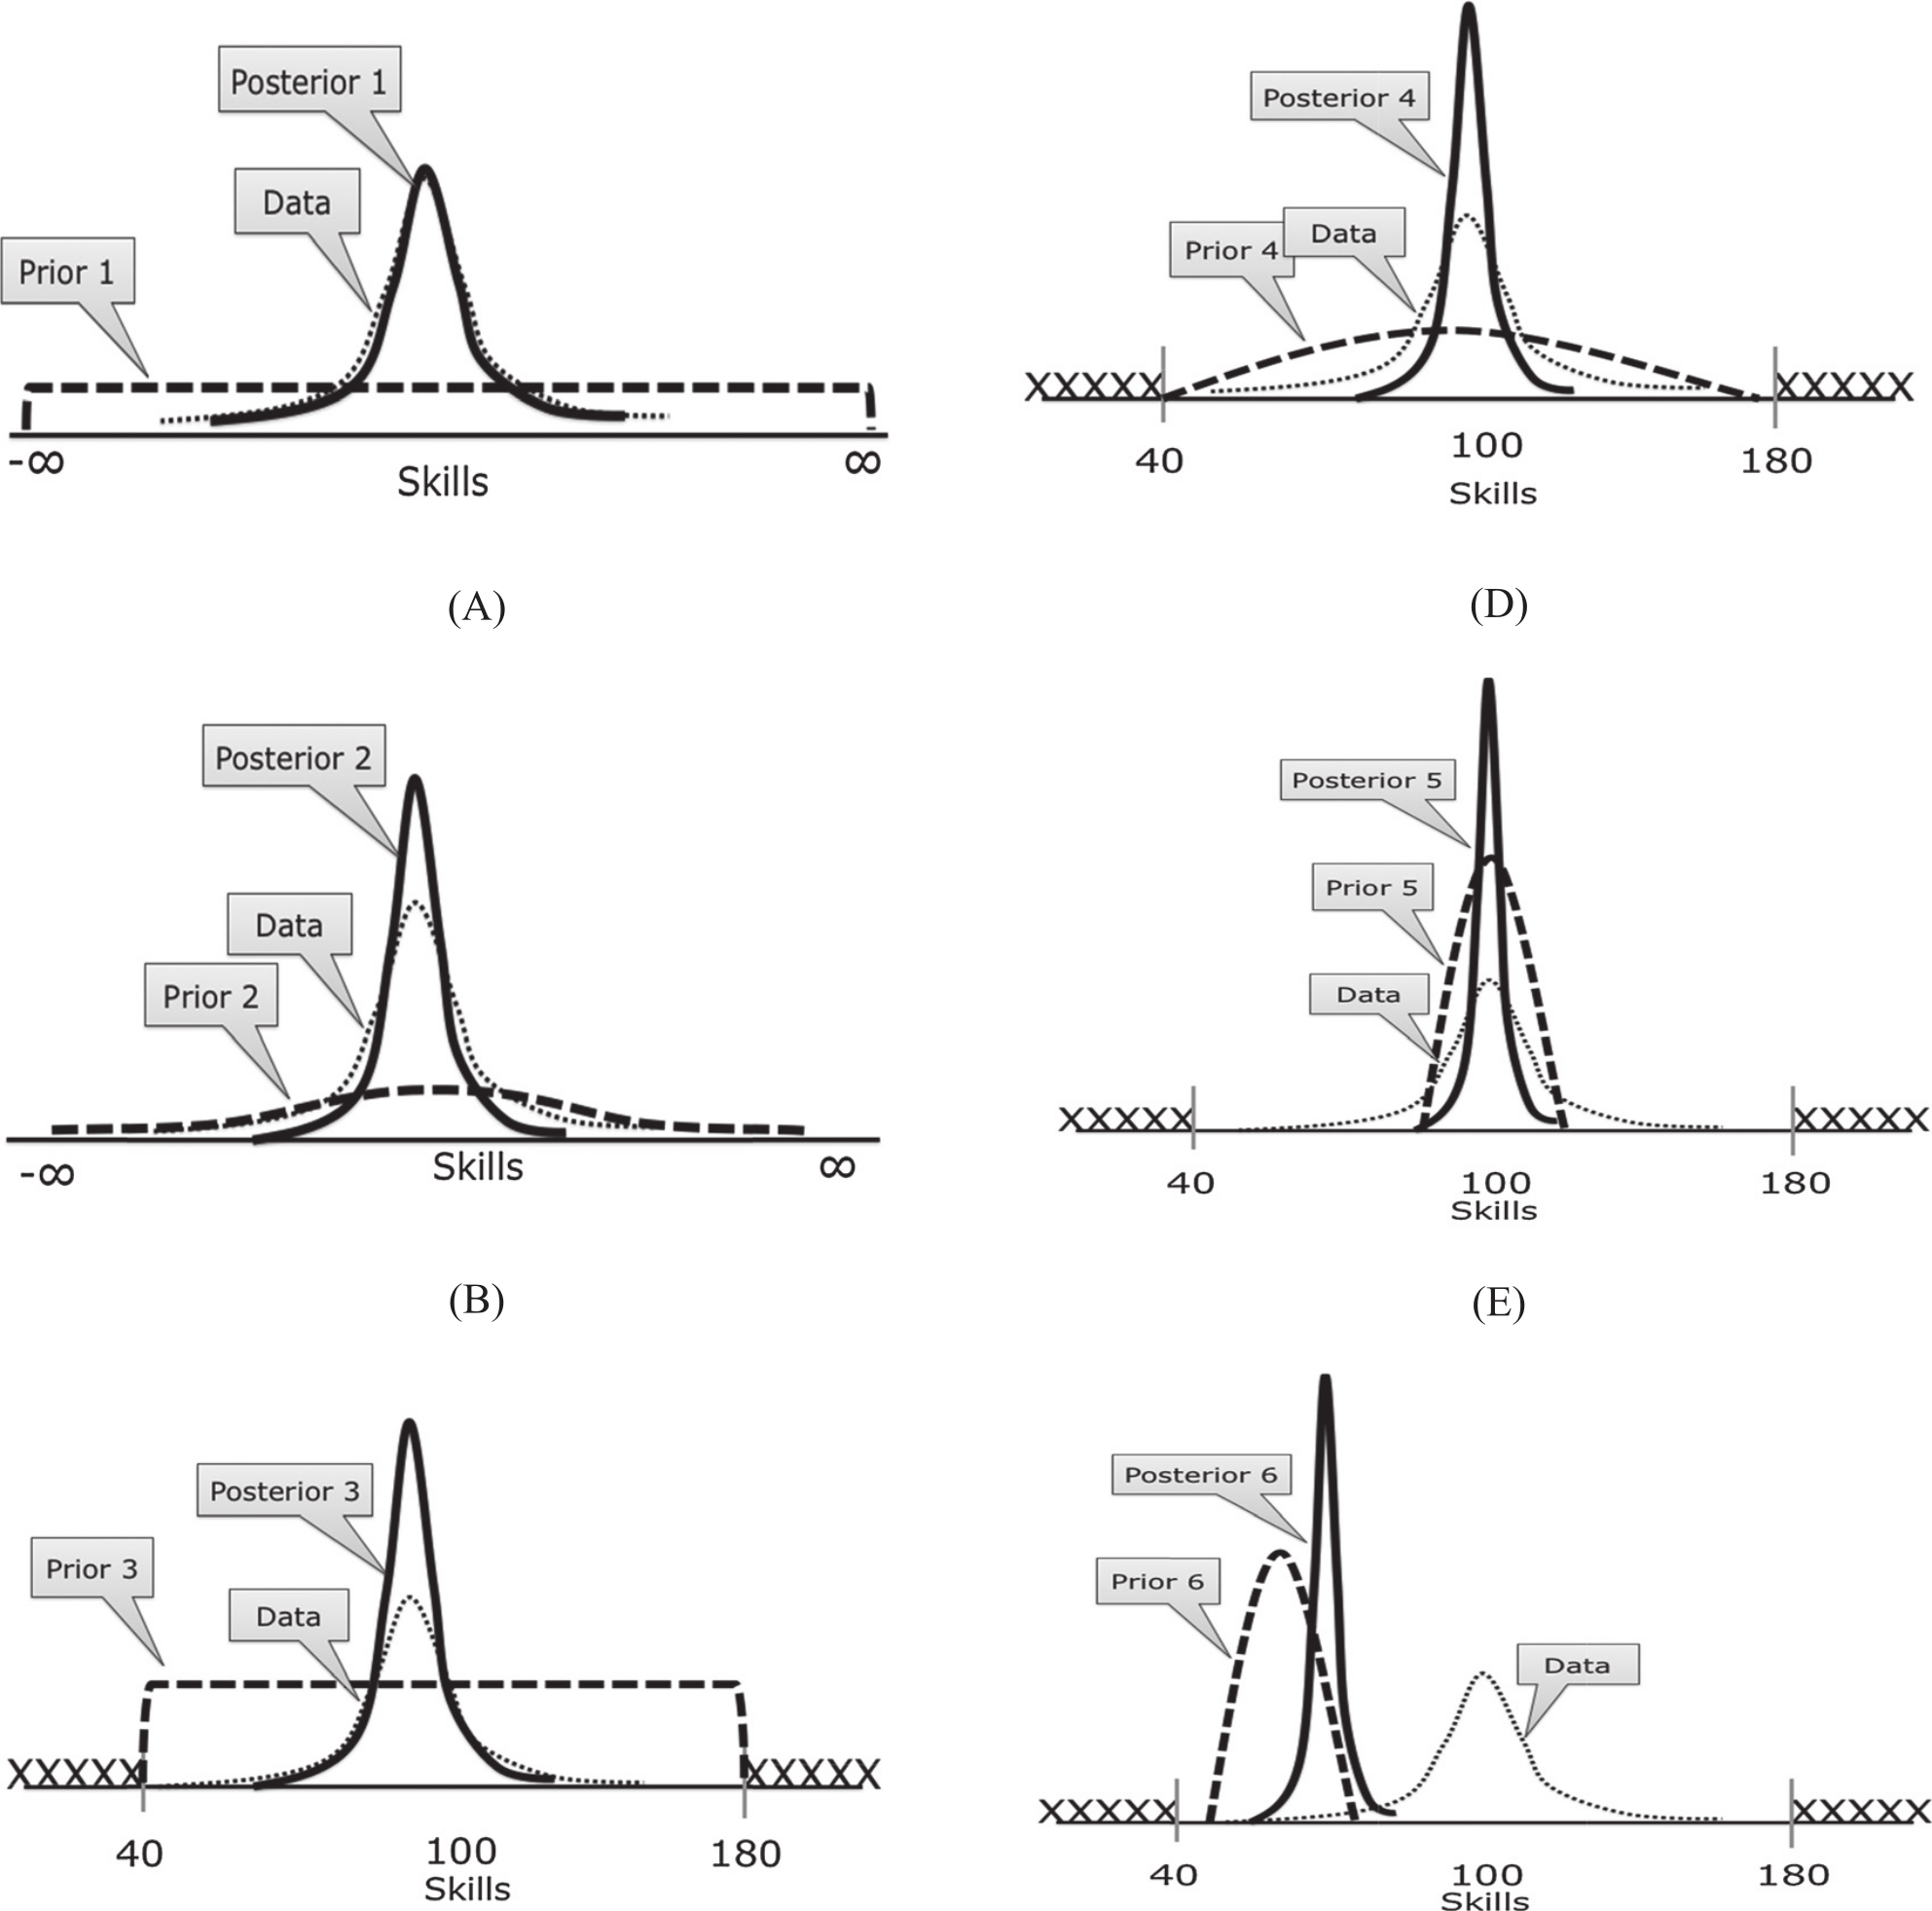
\includegraphics[width=0.7\textwidth]{priors.png}\\
	\scriptsize from van de Schoot \textit{et al.}, 2014
\end{frame}

\begin{frame}{Norms vs Priors}
\begin{itemize}
        \item The median minimize the L1 norm : \\
        $\text{median}(x) = \arg\min_s \sum_i \|x_i - s\|_1$\\
        The least absolute deviation estimate arises from the maximum likelihood estimate with errors having a Laplace distribution\\
        fat-tailed distribution $\rightarrow$ less prone to outliers
        
        $$f=  \| y - Xw \|^2_2 + \lambda_2 \| w \|_1$$
        
        \item The mean minimize the L2 norm : \\
        $\text{mean}(x) = \arg\min_s \sum_i \|x_i - s\|_2$\\
        gives the least squares estimate
        more sensitive to outliers
        
\end{itemize}

\end{frame}


\section{Hierachical Bayesian models}
\begin{frame}{\insertsectionhead}
\textbf{Example:}\\
$$y\mid \theta \sim \N(\theta, 1)$$
\pause
$\theta$ is a parameter of the model. It can have its own distribution (the prior):
$$\theta \mid \mu \sim \N(\mu,1)$$
\pause
$\mu$ is called an hyperparameter. It can also have its own distribution (the hyperprior)
$$\mu \sim \N(0,1)$$
\pause
The full posterior is then:
\begin{align*}
	P(\theta,\mu \mid y) &\propto P(y \mid \theta,\mu)P(\theta,\mu)\\
	& \propto P(y \mid \theta)P(\theta \mid \mu) P(\mu)\\
	&\propto \N(\theta, 1)\N(\mu,1) \N(0,1)
\end{align*}
\pause
If the full posterior does not have a closed-form, it can be approximated by numerical methods such as Monte Carlo Markov Chains. 
\end{frame}
\begin{frame}{\insertsectionhead}
\centering
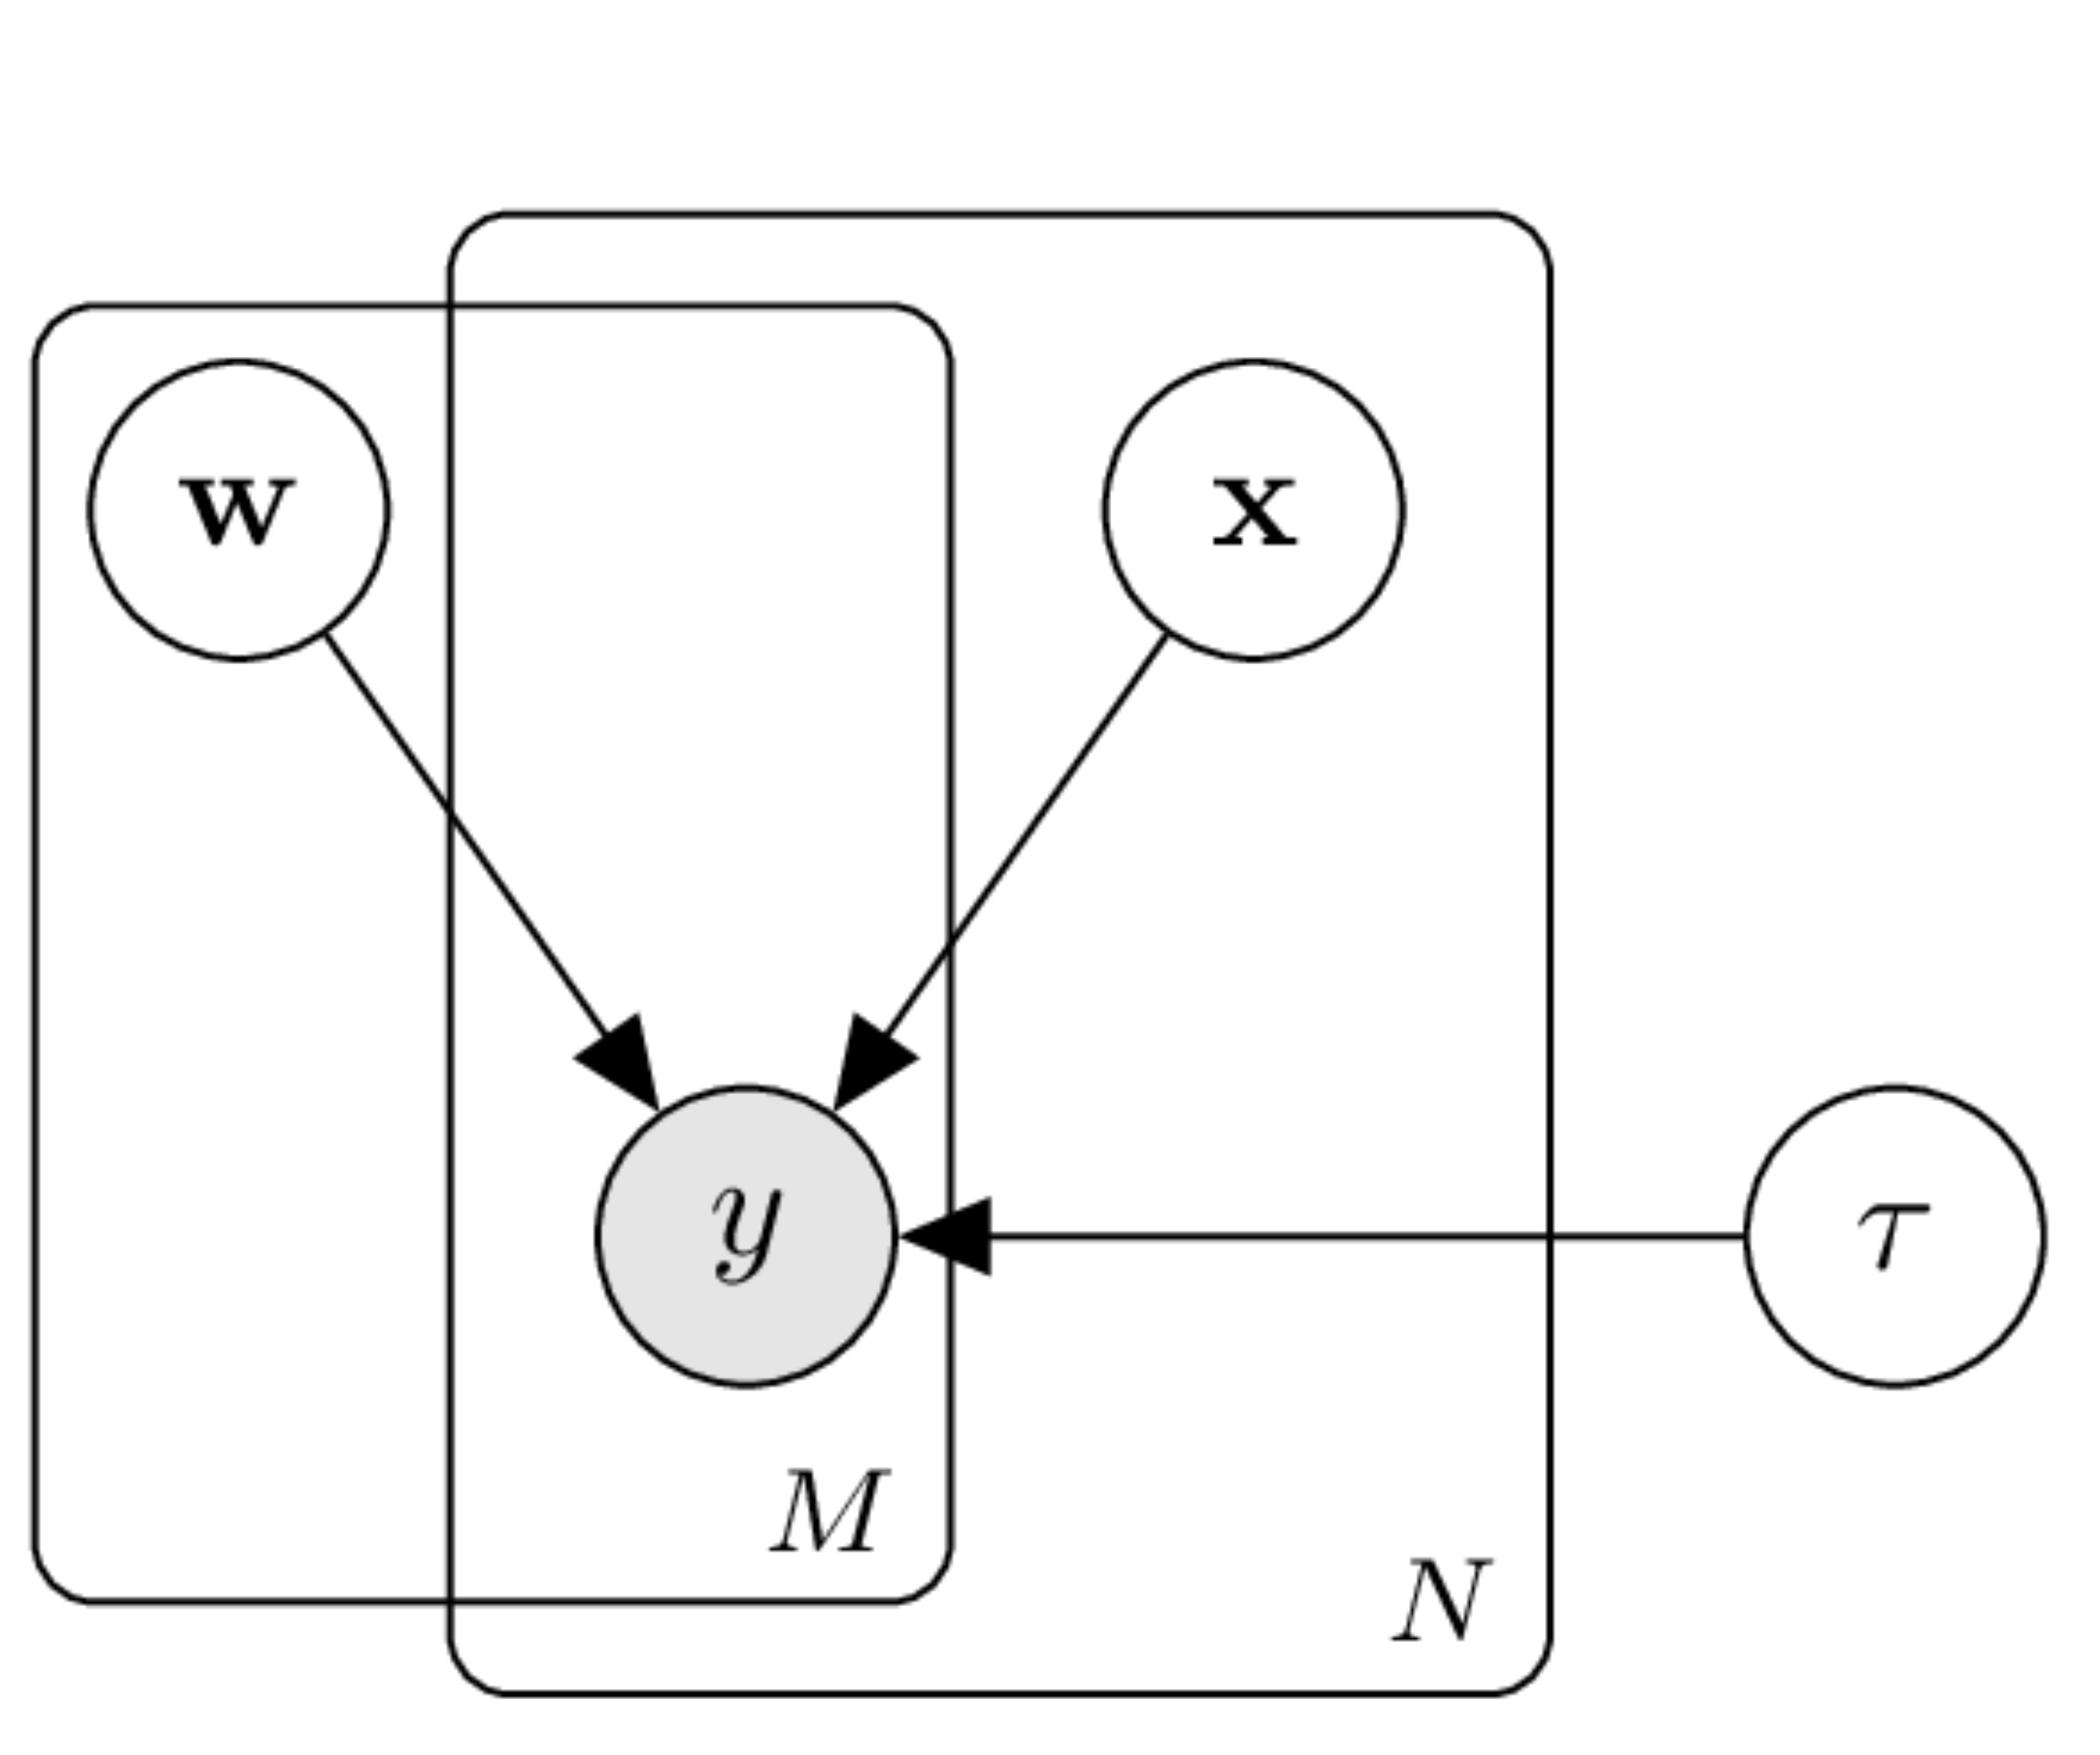
\includegraphics[width=0.5\textwidth]{bayesnet1.png}\\
Read : 
\begin{equation*}
	     y_{m,n} = f_1(w_m) ~ [ + \text{or} \times ]~ f_2(x_n)~ [ + \text{or} \times ]~ f_3(\tau)
\end{equation*}


\vfill
\scriptsize from \texttt{github.com/jluttine/tikz-bayesnet}
\end{frame}

\begin{frame}{\insertsectionhead}
\centering
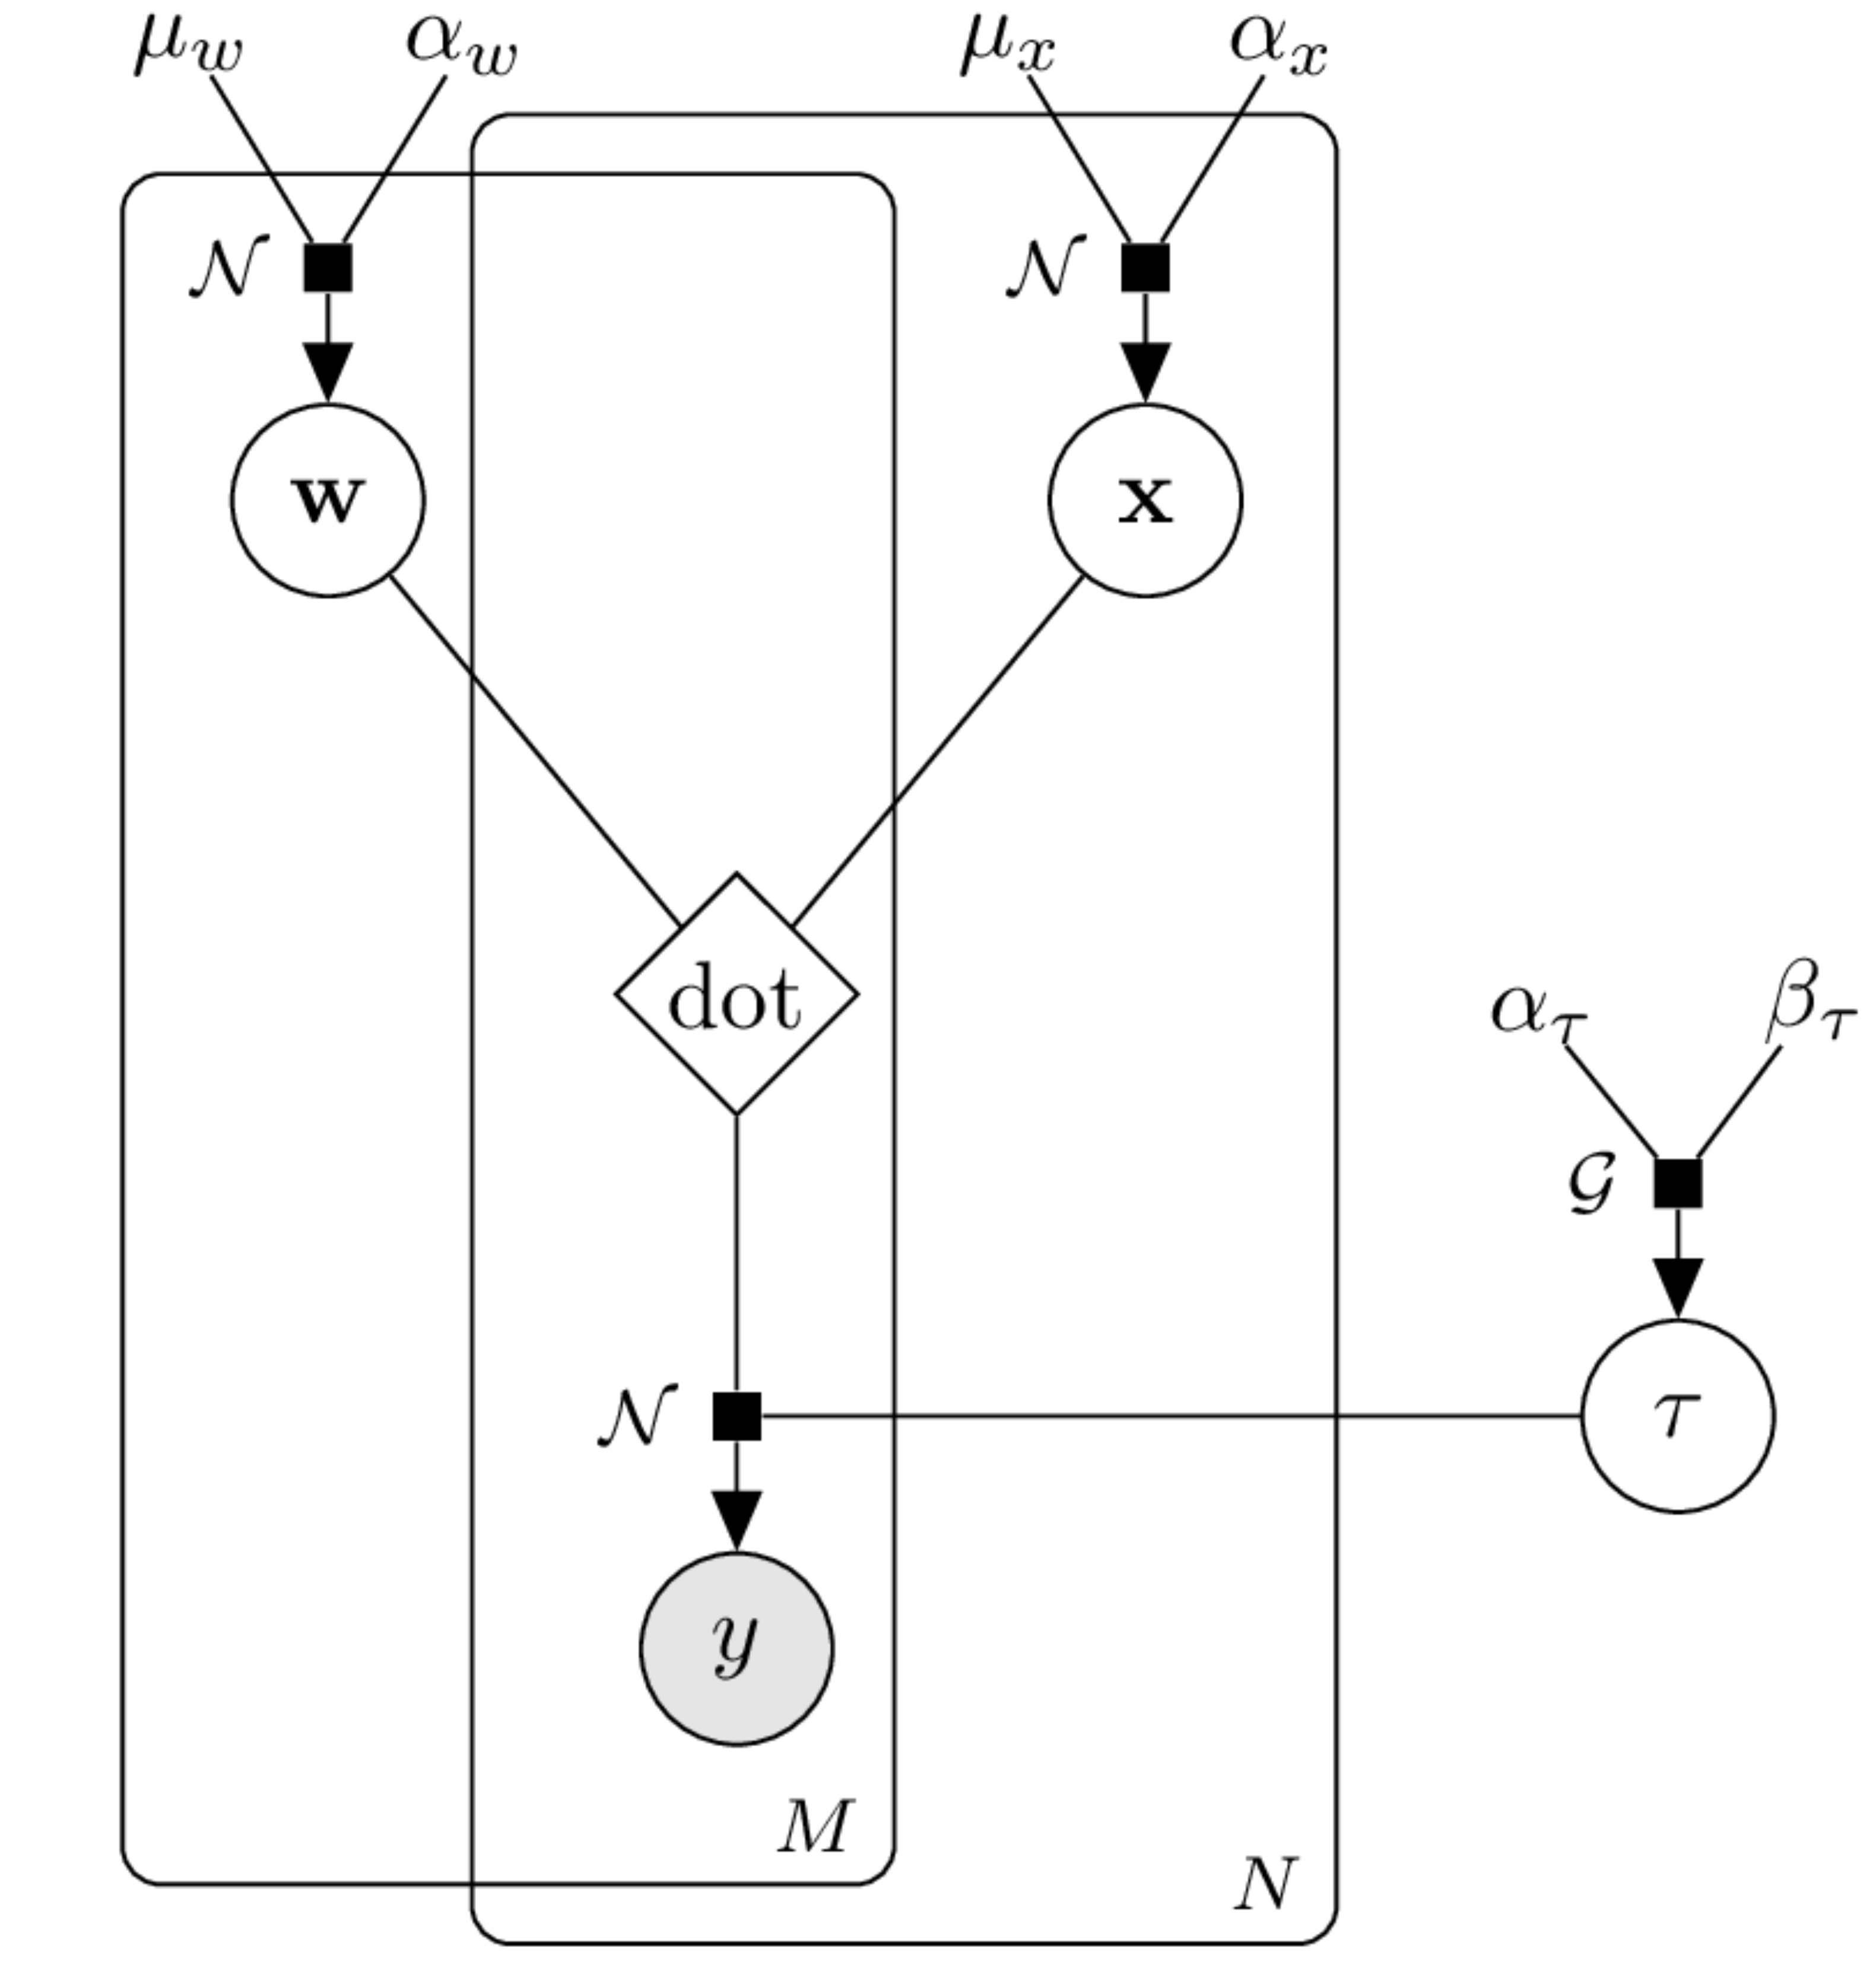
\includegraphics[width=0.5\textwidth]{bayesnet2.png}\\
Read : 
\alt{$$ y_{m,n} = f_1(w_m) \times f_2(x_n) + f_3(\tau)$$}{$$ y_{m,n} = w_m x_n + n$$}
$\hookrightarrow$ Probabilistic Principal Component Analysis model

\vfill
\scriptsize from \texttt{github.com/jluttine/tikz-bayesnet}
\end{frame}



\begin{frame}{Related topics}
\begin{itemize}
	\item Machine learning
        \item Pattern recognition
        \item Neural networks and deep learning
        \item Data mining / Data science
        \item Statistic modeling
        \item Artificial intelligence
\end{itemize}

\textbf{For different fields:}
\begin{itemize}
        \item Engineering (signal processing, system identification, ...)
        \item Computer Science 
        \item Statistics (data science, estimation,...)
        \item Cognitive science and psychology (perception, linguistics,...)
        \item Economics (decision theory, game theory, e-commerce...)
\end{itemize}
\end{frame}


\begin{frame}{References}
Book : \textit{Pattern Recognition and Machine Leaning},  Bishop\\
New article : \textit{Machine learning in acoustics: a review}, Bianco \& coaut.
\end{frame}
\end{document}
